%\question[5]
\begin{myquestion}[10]
    Sam ha dibujado dos paralelogramos. Los midió cuidadosamente y le dijo a Allison que los dos paralelogramos crearían una \emph{rampa de despegue} para el Skatepark. Sam no está seguro de que su diseño funcionará, pero piensa poner un paralelogramo sobre el suelo, luego poner cuatro resortes en el centro y, finalmente, poner el otro paralelogramo encima.

    --Creo que estás loco--, le dijo Allison cuando oyó su idea.

    --¿Eso no importa?, nos pidieron que creáramos una idea única y es única--, respondió Sam.

    --Bueno, entonces ¿tengo que hacer que los lados calcen bien?--.

    --Sí. -- dijo Sam mientras abandonaba la habitación.-- Sólo los lados correspondientes--.
    Allison observó los dos paralelogramos del diseño de Sam. Sabía que necesitaba escribir los lados correspondientes, pero no estaba segura de cómo hacerlo.


    \begin{figure}[H]
        \centering
        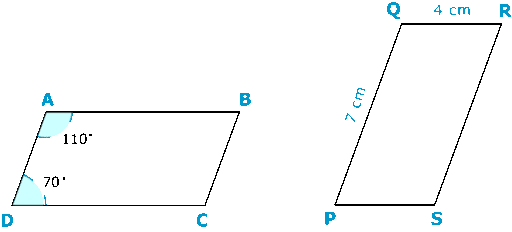
\includegraphics[width=0.45\textwidth]{../images/congruencia01.png}
        \caption{}
        \label{fig:congruencia01}
    \end{figure}

    Estas dos figuras son congruentes. ¿Qué ángulo es congruente al ángulo A?

    \begin{solutionbox}{6cm}
        Debido a que te dijeron que estas dos figuras son congruentes, es importante que no te haga desistir el hecho de que se encuentren en una posición diferente. En tu mente, necesitarás girar la segunda figura, de forma que esté en la misma posición que la primera figura. Si para ti es difícil visualizar esto, también puedes volver a dibujar la figura.

        Aquí está la respuesta:
        \[\angle A \cong \angle P\]
    \end{solutionbox}
\end{myquestion}